\section{Анализ предметной области}

В данном разделе будет произведен краткий обзор существующих аналогов приложения; 
сформулированы требования к разрабатываемому программному средству.

\subsection{Обзор аналогов}

В результате анализа предметной области было выявлено большое количество приложений
по личному учёту доходов и раходов.
В данном подразделе будут приведены три ярких представителя.

Основными критериями сравнения являются: 
\begin{itemize}
  \item пользовательский интерфейс;
  \item удобство и быстрота использования;
  \item возможность категоризации тразакций;
  \item работа со счетами;
  \item возможность просмотра статистики;
  \item отображение текущего состояния счетов.
\end{itemize}

Классическим приложением по учёту доходов и расходов является cистема 
<<Семейный бюджет>>, расположенная по адресу https://koshelek.org.
Данная система предоставляет широкий функционал по контролю личного бюджета.
Предоставляет большие возомжности по генерации отчётов, планированию будущих расходов.
Однако в следствии широких возможностей системы пострадал пользовательский интерфес.
Внешний вид сайта устарел (рисунок \ref{fig:koshelek}), что также сказывается и на 
удобстве использования. Также сайт перегружен множеством вложенных меню и мелких, 
неочевидных иконок, что затрудняет работу с ним неподготовленному пользователю.

\begin{figure}[ht] 
\centering
    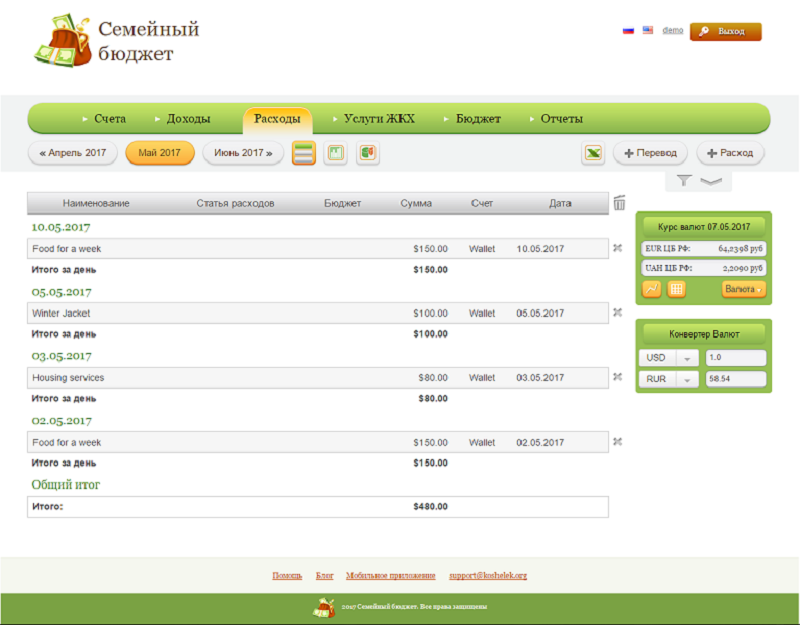
\includegraphics[scale=0.55]{koshelek.png}
    \caption{Раздел <<Доходы>> сайта cистемы <<Семейный бюджет>>}
  	\label{fig:koshelek}
\end{figure}

Кроме этого существует система под названием <<Drebedengi>> расположенная по адресу
http://drebedengi.org (рисунок \ref{fig:drebedengi}). Данная система позволяет
вести учёт доходов и расходов, перемещений между счетами, планировать бюджет и
и контролировать текущее состояние счетов. Также приложение позволяет 
контролировать долги. Пользовательский интерфейс более приятный, по сравнению с
<<Семейным бюджетом>>. Однако всё равно присутствует сложность восприятия из-за
большого количества чисел.

\begin{figure}[p] 
\centering 
    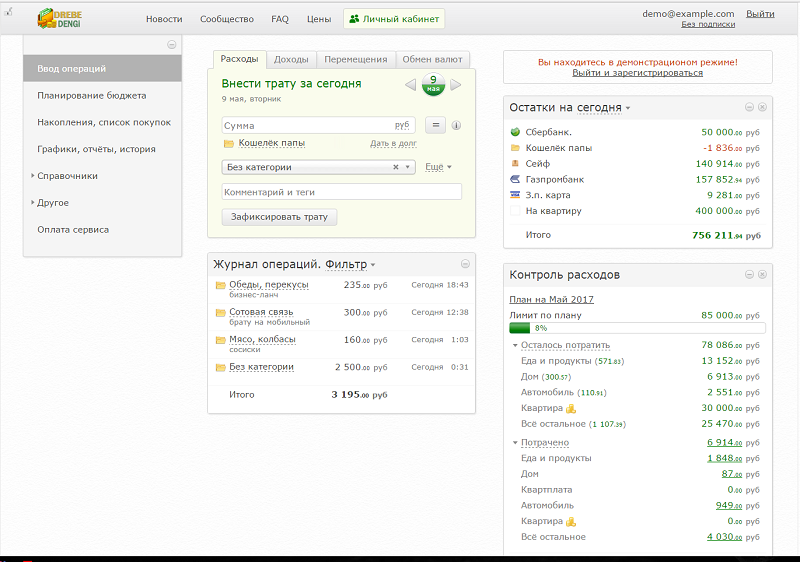
\includegraphics[scale = 0.65]{drebedengi.png}
    \caption{Главная страница пользователя сайта системы <<Drebedengi>>}
    \label{fig:drebedengi}
\end{figure}

Третий аналог, отличающийся от описанных выше отсутсвием перегруженного интерфейса
 --- система <<Zenmoney>> (http://zenmoney.ru). Данное приложение позволяет работать
 с личными счетами, категориями, транзакциями. Предоставляет возможности генерировать
 отчёты, планировать бюджет, просматривать прогноз баланса. Главным недостатком данного \\
 приложения является внешний вид приложение --- большинство элементов интерфейса 
 предоставлены без какой-либо стилизации (рисунок \ref{fig:zenmoney}).

\begin{figure}[p] 
\centering 
    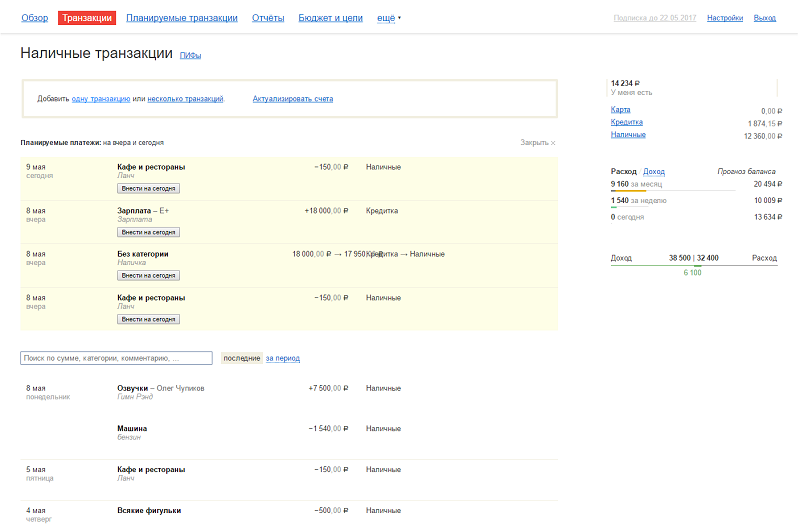
\includegraphics[scale = 0.65]{zenmoney.png}
    \caption{Страница транзакций сайта системы <<Zenmoney>>}
    \label{fig:zenmoney}
\end{figure}

Результат сравнения имеющихся аналогов с разрабатываемым приложением приведён в 
таблице \ref{table:functions_comparing}.

\begin{table}[hb!] \caption{Сравнение приведеных аналогов с
разрабатываемым приложением}
\label{table:functions_comparing}
\centering
     \begin{tabular}{ | >{\centering}m{0.25\textwidth} 
					  | >{\centering}m{0.07\textwidth} 
					  | >{\centering}m{0.19\textwidth} 
					  | >{\centering}m{0.19\textwidth}
					  | >{\centering\arraybackslash}m{0.155\textwidth}|}
	\hline Функция & Kwit & Koshelek.org & Drebedengi.ru & Zenmoney.ru\\
  	\hline Современный интерфейс & + & - & + & -\\
    \hline Простота в использовании & + & - & - & +\\
    \hline Мультивалютность & + & + & + & +\\
    \hline Простота в использовании & + & - & - & +\\
  	\hline Работа со счетами & + & + & + & +\\
  	\hline Работа с категориями & + & + & + & +\\
  	\hline Возможность \\ генерировать отчёты & - & + & + & +\\
  	\hline Прогнозирование & + & + & + & +\\
    \hline
  \end{tabular}
\end{table}


При составлении таблицы учитывался
весь запланированный функционал, реализация некоторых функций возможна в
версиях, которые будут разработаны вне данного курсового проекта.

\subsection{Постановка задачи}

Целью данного курсового проекта является разработка:
\begin{itemize}
  \item добавление, удаление и изменение транзакций;
  \item добавление, удаление и изменение категорий;
  \item добавление, удаление и изменение счетов;
  \item возможность удаления категорий и счетов с переносом всех \\ транзакций на другой счёт;
  \item возмонжость подсчёта статистики по категориям за \\ произвольный период всемени;
  \item подсчёт ежедневной суммы до зарплаты, прогноза будущих затрат \\ за последнее время.
\end{itemize}

Программное средство должно представлять собой сервер c REST API и веб-клиент.
Данное сочетание позволит в дальнейшем развить данное приложение в полноценную
кроссплатформенную систему.